\chapter{Metodologia}

A metodologia concebida para a realização deste trabalho foi classificada quanto à sua natureza, abordagem, objetivos e aos procedimentos técnicos.

Quanto à natureza, a pesquisa possui uma caracterização aplicada, visto que se objetiva gerar conhecimentos de efeito prático e destinados à resolução de problemas específicos. Quanto à abordagem, a pesquisa possui um enfoque qualitativo, devido ao fato de não requerer a utilização de métodos e técnicas estatísticas \cite{metodologia}. Quanto aos objetivos, a pesquisa se caracteriza como descritiva, pois pretende definir um \textit{framework}.

Para concretizar a realização do trabalho, os seguintes procedimentos técnicos foram adotados:

\begin{itemize}
	\item Pesquisa Bibliográfica
	\item Revisão Sistemática
	\item Pesquisa-Ação
\end{itemize}

Pelo fato de o presente trabalho estar centrado na proposição de um \textit{framework} que reúne práticas propostas pela verificação de \textit{software} e integra estas às diretrizes fornecidas pela VBSE, fez-se necessária a seleção de mais de um procedimento técnico de pesquisa para a construção do trabalho.
 
O arcabouço teórico inerente à VBSE e às inspeções de código foi obtido a partir da pesquisa bibliográfica.

Para Fonseca (2002), a pesquisa bibliográfica é realizada a partir do levantamento de referências teóricas já analisadas, e publicadas por meios escritos e eletrônicos. A pesquisa bibliográfica possibilita que o pesquisador conheça o que já se estudou sobre a temática.

Também foi utilizada como fonte para o estabelecimento do \textit{framework} uma revisão sistemática de literatura sobre qualidade de implementação de testes unitários, realizada na disciplina Engenharia de \textit{Software} Experimental do curso de graduação em Engenharia de \textit{Software} da Faculdade UnB Gama (FGA). 

A revisão sistemática, por sua vez, se estabelece como uma metodologia bem definida para identificar, analisar e interpretar as melhores abordagens e práticas relacionadas a uma determinada questão de pesquisa \cite{sistematica}. Além desses aspectos, é uma metodologia que possibilita uma repetição concisa.

A opção pelo uso desta revisão sistemática deve-se ao fato de que este trabalho também está voltado para a tentativa de compreender quais têm sido as abordagens empregadas na elaboração de testes unitários e como se tem avaliado a efetividade destes. O \textit{framework}, naturalmente, compreende a prática de elaboração de testes unitários.

Outro aspecto interessante da revisão sistemática é que esta auxilia de maneira precisa na localização dos principais trabalhos publicados para uma determinada problemática, favorecendo a construção de uma linha cronológica que demonstra ao pesquisador quais linhas têm sido defendidas e quais são os campos mais promissores para uma futura exploração.

\section{Detalhamento do Plano Metodológico}

O plano metodológico concebido para a formulação e aplicação do \textit{framework} aqui proposto se subdivide em duas partes, sendo a primeira atrelada ao TCC 1 (Trabalho de Conclusão de Curso 1) e a segunda, ao TCC 2.

A primeira parte compreende 3 fases: \textit{Planejamento da Pesquisa}; \textit{Coleta de Informações} e \textit{Proposta de Solução}.

A fase inerente ao \textit{Planejamento da Pesquisa} envolve a definição de objetivos, pergunta de pesquisa, classificação metodológica e estabelecimento dos procedimentos técnicos de pesquisa. É válido evidenciar que essas definições são realizadas a partir do problema que foi identificado.

A fase de \textit{Coleta de Informações} compreende a aplicação dos procedimentos técnicos adotados para a pesquisa, que para este trabalho foram a pesquisa bibliográfica e a revisão sistemática.

Por fim, na fase \textit{Proposta de Solução}, há a concepção de uma possível solução para a problemática identificada. Esta solução, por sua vez, está embasada nas informações coletadas na fase anterior.

A figura \ref{fig:plano1} ilustra essa parte do plano metodológico.

\begin{figure}[h]
\includegraphics[width=\textwidth]{figuras/planometodologico1.png}
\caption{Plano Metodológico - TCC 1}
\label{fig:plano1}
\end{figure}

\clearpage

A segunda parte, já vinculada ao TCC 2, e voltada para a implantação e avaliação da proposta, envolve outras 3 fases: \textit{Coleta de Dados}; \textit{Análise e Interpretação dos Resultados} e \textit{Divulgação dos Resultados}, conforme ilustrado na Figura 2.
A fase \textit{Coleta de Dados} envolve a aplicação de um procedimento técnico denominado pesquisa-ação. Esse procedimento possibilita que o pesquisador intervenha dentro da problemática, mobilizando os participantes e construindo novos conhecimentos \cite{pesquisa}. Assim, a cada ciclo novos quesitos poderão ser melhor tratados no \textit{framework}.

Na fase \textit{Análise e Interpretação dos Resultados}, todos os dados coletados a partir da utilização do \textit{framework} serão analisados, de forma que todas as percepções possíveis possam ser obtidas. Por fim, na fase \textit{Divulgação dos Resultados}, haverá uma estruturação de todos os dados obtidos e analisados, de forma que possa ser evidenciado a efetividade do uso do \textit{framework}.

A figura \ref{fig:plano2} ilustra a segunda parte do plano metodológico.

\begin{figure}[h]
\includegraphics[width=\textwidth]{figuras/planometodologico2.png}
\caption{Plano Metodológico - TCC 2}
\label{fig:plano2}
\end{figure}

\section{Elaboração da Proposta do \textit{Framework}}

A primeira parte do plano metodológico foi executada durante a realização do TCC 1. Com base no problema identificado e nas informações levantadas por meio da pesquisa bibliográfica e da revisão sistemática, foi possível conceber o \textit{framework} de verificação estática e dinâmica de código. Adicionalmente, já foi definido como a avaliação do \textit{framework} seria feita. As próximas seções descrevem detalhadamente este quesito que, por sua vez, constitui a segunda parte do plano metodológico, executado durante este trabalho (TCC 2).

\section{Estratégia de Aplicação do \textit{Framework}}

Antes da incorporação das atividades propostas pelo \textit{framework} à rotina das organizações utilizadas como casos, foi feita uma reunião com os principais envolvidos de cada projeto. Assim, foram explicitados todos os aspectos do \textit{framework} e a importância dessas atividades para que haja aumento na qualidade do \textit{software}.

Adicionalmente, foi construída uma página na wiki dos ambientes dos projetos que dispõe da imagem do processo que constitui o \textit{framework}, bem como o detalhamento deste, de forma que os \textit{stakeholders} dos projetos pudessem efetuar consultas em caso de dúvidas.

Como mencionado em seção anterior, a pesquisa-ação foi o procedimento técnico empregado para analisar o uso do \textit{framework}.

\section{Organizações onde o \textit{Framework} foi aplicado}

\subsection{Controladoria Geral do Distrito Federal}

A Controladoria Geral do Distrito Federal (CGDF) teve sua estrutura criada por meio do Decreto nº 36.236, de 1º de janeiro de 2015, pelo Governador Rodrigo Rollemberg. Esta Unidade Gestora possui como missão orientar e controlar a gestão pública, com transparência e participação da sociedade.

Interna à CGDF há uma coordenação, a COTEC (Coordenação de Administração de Assuntos Tecnológicos), que é responsável por desenvolver e manter sistemas para todas as demais coordenações da CGDF. Além dos sistemas internos, tem-se aplicações que são desenvolvidas por empresas privadas ao governo e entregues à COTEC para serem mantidas.

A equipe da COTEC é pequena, contando com um total de 10 servidores. São 3 servidores na frente de infraestrutura, 3 na frente de administração de banco de dados e apenas 4 na área de desenvolvimento. O \textit{Scrum} e XP foram adotados recentemente na COTEC.

A maior parte dos sistemas desenvolvidos e mantidos pela COTEC são aplicações \textit{Web}, construídas com as linguagens de programação \textit{CSharp}, Java e \textit{Ruby} com auxílio do \textit{framework} \textit{Rails}. Adicionalmente, faz-se uso do \textit{framework} \textit{AngularJS} para elaboração da camada de apresentação das aplicações.

Embora já se tenha o mínimo de atividades para controlar o desenvolvimento, a COTEC ainda necessita incorporar uma série de outras práticas. As atividades inerentes à verificação de \textit{software} ainda são incipientes na COTEC, tornando-a um local propício para a aplicação do \textit{framework}.

\subsection{Laboratório Fábrica de \textit{Software} - Campus UnB Gama}

O Laboratório Fábrica de \textit{Software} foi concebido com fins de pesquisa e promoção de excelência no desenvolvimento de \textit{software}. Atualmente, o laboratório já incorpora metodologias ágeis para o desenvolvimento, sendo o \textit{Scrum} e o XP (\textit{Extreme Programming}).

Adicionalmente, o laboratório atua de forma a unir o aprendizado das disciplinas do curso de Engenharia de \textit{Software} do Campus Gama da UnB, e a atuação prática de projetos reais.

O laboratório possui parceria com instituições públicas e privadas, as quais subsidiam pesquisas e projetos utilizando tecnologia \textit{CSharp} e \textit{Android}. Quando necessário, o laboratório também modela processos de negócio utilizando notação BPMN (\textit{Business Process Model and Notation}).

Por se tratar de uma instituição aberta ao âmbito de pesquisa na área de Engenharia de \textit{Software}, o laboratório é um local apropriado para uso e experimentação do \textit{framework}, justamente pelo fato de conciliar interesses práticos do mercado com os fins acadêmicos.

\section{Avaliação da Efetividade do \textit{Framework}}

Para realizar uma análise da efetividade da aplicação do \textit{framework}, elaborou-se um GQM (\textit{Goal Question Metrics}) \cite{gqm}. A seguir, tem-se a tabela \ref{table:tabela1}, que resume o objetivo da medição.

\begin{table}[h]
\caption{Tabela Resumo do Objetivo de Medição}
\centering
\begin{tabular}{ | m{8cm} | m{8cm} | } 
\hline
Analisar & A aplicação do \textit{framework} \\ 
\hline
Com o propósito de & Melhorar \\ 
\hline
Com respeito a & Efetividade do \textit{framework} \\ 
\hline
Sob o ponto de vista de & \textit{Stakeholders} do projeto \\ 
\hline
No contexto de & Projetos de desenvolvimento e manutenção da Fábrica e da Controladoria \\ 
\hline
\end{tabular}
\label{table:tabela1}
\end{table}

\hfill \break

\hfill \break

A partir do quadro resumo que descreve o objetivo de medição, foram elaboradas questões a serem respondidas por meio das medições, bem como as métricas associadas às mesmas. A seguir, tem-se a apresentação das questões e métricas.

\begin{itemize}
	\item \textbf{Questão 1:} Como a quantidade de defeitos do código fonte evolui ao longo das \textit{sprints}?
	\subitem Número de Defeitos encontrados em Inspeções

	\item \textbf{Questão 2:} Qual o nível de eficácia dos testes unitários implementados a partir do uso do guia de implementação do \textit{framework}?
	\subitem Taxa de acertos por linha de código (Métrica fornecida pelas ferramentas de análise de cobertura)

	\item \textbf{Questão 3:} Qual o número de falhas reportados pelos usuários após homologação da \textit{release} entregue?
	\subitem Número de Falhas em Produção

	\item \textbf{Questão 4:} Qual o grau de satisfação dos desenvolvedores ao utilizarem os guias de inspeção e de implementação de testes unitários propostos pelo \textit{framework}?
	\subitem Índice de Satisfação dos Desenvolvedores

	\item \textbf{Questão 5:} Qual o grau de facilidade percebido quando vai ser feita uma manutenção no código?
	\subitem Índice de Manutenibilidade (Para Java e \textit{CSharp}) e Flog (para \textit{Ruby})
\end{itemize}

As métricas relacionadas às questões 4 e 5 são detalhadas a seguir.

A coleta de métricas foi realizada ao final de cada \textit{sprint}, de maneira a avaliar os resultados e verificar a efetividade do \textit{framework}. Caso ajustes fossem necessários, as modificações eram feitas e novamente, todo o ciclo de atividades era executado na \textit{sprint} seguinte.

Adicionalmente, para o correto uso do \textit{framework}, foi proposta uma etapa a mais no kanban de implementações da equipe de desenvolvimento, sendo esta a inspeção de código. A funcionalidade só seria considerada finalizada, após inspecionada e aprovada por outro integrante da equipe.

\section{Pesquisa de Satisfação dos Desenvolvedores}

Para verificar o nível de satisfação dos desenvolvedores, concebeu-se uma pequena lista com itens a serem julgados pelos desenvolvedores de acordo com as opções disponíveis, citadas como componentes da métrica que responde à questão 4. A seguir, tem-se os itens de pesquisa.

\begin{itemize}
	\item As inspeções de código se mostraram eficazes na identificação de defeitos no código?

	\item Os testes unitários implementados de acordo com o guia, de fato, exercitam o código de maneira eficiente?

	\item As inspeções de código efetuadas segundo o guia e as implementações de testes unitários também feitas de acordo com o guia demonstraram-se onerosos ao processo de desenvolvimento?

	\item O número de falhas percebidos pelo usuário passou a ser menor a cada \textit{release} entregue?

	\item A manutenibilidade do código ficou melhor após as inspeções de código?
\end{itemize}

Realizou-se o cômputo das respostas atribuídas pelos desenvolvedores aos itens da pesquisa de satisfação usando a escala \textit{Likert}: 

\begin{itemize}
	\item {1 - Concordo Totalmente}.
	\item {2 - Concordo Parcialmente}.
	\item {3 - Neutro}.
	\item {4 - Discordo Parcialmente}.
	\item {5 - Discordo Totalmente}.
\end{itemize}

É importante ressaltar que a pesquisa foi aplicada ao final de cada \textit{sprint}. Dessa maneira, os desenvolvedores puderam assimilar mais experiências para fornecerem respostas mais concisas ao julgar os itens da pesquisa.

Por fim, com relação ao índice de satisfação dos desenvolvedores, nenhuma fórmula específica foi desenvolvida. Considerou-se o percentual das alternativas da Escala \textit{Likert} obtido para cada questão do questionário.

\section{Índice de Manutenibilidade e Flog}

Com relação às métricas adotadas por meio da aplicação do GQM, citadas anteriormente, esta seção traz detalhes acerca do Índice de Manutenibilidade.

O Índice de Manutenibilidade indica um valor entre 0 e 100 e representa a facilidade em manter o código de um determinado módulo. Um valor alto expressa melhor manutenibilidade. De acordo com o portal de métricas de código fonte da \textit{Microsoft}, disponível em (https://msdn.microsoft.com/pt-br/library/bb385914.aspx), valores entre 20 e 100 expressam boa manutenibilidade. Valores entre 10 e 19 indicam manutenibilidade moderada e, por fim, valores entre 0 e 9 indicam pouca manutenibilidade.

A figura \ref{fig:formulaManutenibilidade} expressa a fórmula utilizada para calcular o Índice de Manutenibilidade, que foi concebida por Paul Oman e Jack Hagemeister e apresentada pela primeira vez em 1992 na ICSM (\textit{International Conference on Software Maintenance}).

\begin{figure}[h]
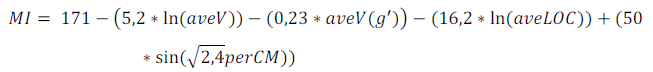
\includegraphics[width=\textwidth]{figuras/mi.png}
\caption{Fórmula para o cálculo do Índice de Manutenibilidade}
\label{fig:formulaManutenibilidade}
\end{figure}

A fórmula considera o Volume de Halstead, que indica a facilidade de entender o código, considerando todos os operadores e operandos, a complexidade ciclomática, que expressa a quantidade de fluxos diferentes que podem ser obtidos, a quantidade de linhas de código e o percentual de linhas de comentário.

Com relação aos projetos em \textit{Ruby}, foi necessário selecionar uma métrica mais apropriada para avaliar a manutenibilidade do código (Flog), pois o recurso de metaprogramação, fortemente presente em código \textit{Ruby}, acrescenta particularidades para a análise de manutenibilidade.

A métrica Flog expressa uma pontuação que é fornecida ao código com base em três quesitos:

\begin{itemize}
	\item Atribuições: quanto mais atribuições são feitas, maior é a pontuação obtida.
	\item Ramos (\textit{Branches}): quando o código se ramifica, existem vários caminhos que podem ser seguidos. Esse aspecto aumenta a complexidade do código.
	\item Chamadas: a quantidade de chamadas efetuadas internamente entre os módulos afeta a complexidade do código, visto que existem muitas interfaces e passagens de parâmetros.
\end{itemize}

Para cada um dos quesitos citados acima há uma pontuação diferente associada. Por exemplo, uma chamada de método padrão recebe pontuação igual a 2, mas uma chamada \textit{eval} já recebe pontuação igual a 5, mesmo que ambos sejam chamadas. Quanto mais complexo for o entendimento do código, mais alta será a pontuação. Há um site que contem a lista de pontuações categorizada para a métrica disponível em (http://docs.seattlerb.org/flog/). Com relação ao nível de aceitação proposto pelos idealizadores da métrica, um método com boa aceitação possui pontuação total inferior à 40.